
\documentclass[a4paper, 12pt,oneside,toc=chapterentrywithdots]{scrbook}

\usepackage[english]{babel}
\usepackage[backend=biber, style=numeric-comp]{biblatex}
\usepackage[utf8]{inputenc}
\usepackage[T1]{fontenc}
\usepackage[onehalfspacing]{setspace}
\usepackage{ragged2e}
\usepackage{graphicx}
\usepackage{tabularx}
\usepackage[left=2.5cm,right=2.5cm,top=2.5cm,bottom=2.5cm,includeheadfoot]{geometry}
\usepackage{acronym}
\usepackage{nameref}
\usepackage{appendix}
\usepackage{eurosym}
\usepackage[bookmarks=true, pdfborder={0 0 0}]{hyperref}
\usepackage[figure]{hypcap}
\usepackage{makecell}
\usepackage{enumitem}
\usepackage{amssymb}
\usepackage{fancyvrb}
\usepackage{color}
\usepackage[dvipsnames]{xcolor}
\hypersetup{
    colorlinks=true, 
    linkcolor=black,
    anchorcolor=black,
    citecolor=black, 
    filecolor=black,
    urlcolor=blue
}
\usepackage{listings}
\usepackage{tikz}
\usetikzlibrary{shapes, arrows}
\tikzstyle{terminator} = [rectangle, draw, text centered, rounded corners, minimum height=2em]
\tikzstyle{process} = [rectangle, draw, text centered, minimum height=2em]
\tikzstyle{decision} = [diamond, draw, text centered, minimum height=2em]
\tikzstyle{data}=[trapezium, draw, text centered, trapezium left angle=60, trapezium right angle=120, minimum height=2em]
\tikzstyle{connector} = [draw, -latex']
% \tikzstyle{arrow} = [thick,->,>=stealth]
\tikzstyle{arrow} = [draw, -latex']


%\usepackage{scrpage2}
%\pagestyle{scrheadings}
%\clearscrheadfoot


\sloppy
\setlength{\parindent}{0pt}
\setlength{\parskip}{1.5ex plus0.0ex minus0.0ex}

\renewcommand*{\arraystretch}{1.5}
\newcommand{\kursiv}[1]{\emph{#1}}
\renewcommand*{\headfont}{\normalfont}
\renewcommand*\chapterheadstartvskip{\vspace*{-1.5cm}}
\renewcommand*\chapterheadendvskip{\vspace*{0.4cm}}
\RedeclareSectionCommands[
beforeskip=-.1\baselineskip,
afterskip=.25\baselineskip
]{section,subsection,subsubsection}

%\DeclareNameAlias{sortname}{last-first}
%\DeclareNameAlias{default}{last-first}

\pagestyle{headings}

\let\origappendix\appendix
\renewcommand\appendix{\clearpage\pagenumbering{roman}\setcounter{page}{\value{anhangcounter}}\origappendix}
\makeatletter
\renewcommand*{\@pnumwidth}{3em}
\renewcommand*{\@tocrmarg}{7em}
%\g@addto@macro\appendix{%
%	\counterwithin*{lstlisting}{section}%
%}
\makeatother
\clubpenalty = 10000
\widowpenalty = 10000

%Quelltextverzeichnis
% \renewcommand{\lstlistingname}{Quelltext}
% \renewcommand{\lstlistlistingname}{Quelltextverzeichnis}

\addbibresource{Bibliography.bib}


\begin{document}

	
	\frontmatter
	
	% \def\title{Re-implementation of a VBA application for calculations according to DIN in Java}
\def\title{ball-bearings-with-quarkus Project}
\def\abgabe{xx.xx.2023}

\begin{titlepage}
	
	
	
	\vspace{5pt}
	
	\begin{center}
		
		\Large \textbf\title
		
		\vspace{50pt}
		
		\large T3\_3101
		
		by 
		
		\large \textbf{Timo Max} 
		
		\vspace{15pt}
		
		in 
		
		\large computer science course
		
		Duale Hochschule Baden-Württemberg Mosbach

        \vspace{10pt}

        
\includegraphics[height=3.5cm]{images/dhbw-logo.jpg}
		
		\vspace{20pt}
		
		\large submitted: \abgabe
		
		\vspace{30pt}

		
		\begin{table}[h]
			\centering
			\begin{tabular}{r l}
				\large\textbf{matriculation number, class} & \large 4706893, MOS-INF20B \\
                \large\textbf{expert} & \large Philipp Abele \\
			\end{tabular}
			
		\end{table}
		
	\end{center}
	
	
\end{titlepage}
	
	\chapter*{Erklärung der Eigenständigkeit}

\begin{justify}
	\large Ich versichere hiermit, dass ich meine Studienarbeit mit dem Thema \kursiv{\title} selbstständig verfasst und keine anderen als die angegebenen Quellen und Hilfsmittel benutzt habe.
	
	\vspace{15pt}
	
	%		\large \noindent Ich versichere zudem, dass die eingereichte elektronische Fassung mit der gedruckten Fassung übereinstimmt.
	
	\vspace{25pt}
	
	\noindent 
	\begin{tabular}{lp{2em}l}
		
		Mosbach, \abgabe  && \hspace{6cm} \\\cline{1-1}\cline{3-3}
		
		Ort, Datum     && Unterschrift
		
	\end{tabular}
	
\end{justify}
	
	\chapter*{Abstract}

	\section*{English}
		
		

	\section*{German}
		
	
	\tableofcontents
	
	\cleardoublepage
	\phantomsection\addcontentsline{toc}{chapter}{List of Abbreviations}
	\chapter*{List of Abbreviations} 

\begin{acronym}
	
	% alphabetisch sortieren 
	\acro{api}[API]{Application Programming Interface}
	\acro{apt}[APT]{Advanced Packaging Tool}
	\acro{bash}[Bash]{Bourne-again shell}
	\acro{cli}[CLI]{Command Line Interface}
	\acro{gpg}[GPG]{GNU Privacy Guard}
	\acro{rsa}[RSA]{Rivest–Shamir–Adleman}
	\acro{vba}[VBA]{Visual Basic for Applications}
	\acro{vo}[vo]{value objects}
	
	
\end{acronym}
	
	\cleardoublepage
	\phantomsection\addcontentsline{toc}{chapter}{\listfigurename}
	\listoffigures
	
	\cleardoublepage
	\phantomsection\addcontentsline{toc}{chapter}{\listtablename}
	\listoftables
	
	% \cleardoublepage
	% \phantomsection\addcontentsline{toc}{chapter}{Quelltextverzeichnis}
	% \lstlistoflistings
	
	\newcounter{anhangcounter}
	\setcounter{anhangcounter}{\value{page}}
	\stepcounter{anhangcounter}
	
	\mainmatter
	
	% some settings
\nocite{*}
\lstdefinestyle{bash}{basicstyle=\ttfamily, columns=fullflexible, language=bash, breaklines=true, showspaces=false, showstringspaces=false, breakatwhitespace=true} 

  
\chapter{Introduction} 
    The microservice will be about a calculation process for ball bearings in O-assignment. The aim is to calculate the lifetime of the O-arrangement in hours (see \textit{lh10} in class OArrangement in \ref{sec:class_diagram}). \\ 

    \section{Flow chart for calculation process}
        The necessary steps for calculating the lifetime of two ball bearings in O-assignment are shown in the following flow chart.   
        
        \begin{tikzpicture}[node distance = 2cm]
            \node [terminator, fill=blue!20] (start) {\textbf{Start}};
            \node [process, fill=blue!20, below of=start] (conversion) {conversion of geometric measures};
            \node [process, fill=blue!20, below of=conversion] (radial) {calculation of radial forces};
            \node [process, fill=blue!20, below of=radial] (axial) {calculation of axial forces};
            \node [process, fill=blue!20, below of=axial] (equivalent) {calculation of dynamic equivalent bearing load};
            \node [process, fill=blue!20, below of=equivalent] (lifetime) {calculation of bearing lifetime};
            \node [data, fill=blue!20, below of=lifetime] (result) {lifetime of bearing in hours};
            \node [terminator, fill=blue!20, below of=result] (end) {\textbf{End}};

            \path [connector] (start) -- (conversion);
            % \draw [arrow] (decision) -- node[anchor=east] {yes} (conversion);
            % \draw [arrow] (decision) -- node[anchor=south] {no} (einschaltdauer);
            \path [connector] (conversion) -- (radial);
            \path [connector] (radial) -- (axial);
            \path [connector] (axial) -- (equivalent);
            \path [connector] (equivalent) -- (lifetime);
            \path [connector] (lifetime) -- (result);
            \path [connector] (result) -- (end);
        \end{tikzpicture}

    \section{Class diagram} \label{sec:class_diagram}
        The underlying data model consists of 3 classes: \textit{Bearing}, \textit{OArrangement} and \textit{Load}. 

        \begin{tikzpicture}
            \begin{class}[text width=8cm]{Bearing}{0,0}
                \attribute{- cdyn : double}
                \attribute{- y : double}
                \attribute{- e : double}
                \attribute{- xB1 : double}
                \attribute{- p: double}
                \attribute{- fr: double}
                \attribute{- fa: double}
                \attribute{- lh10: double}
            \end{class}
        \end{tikzpicture}

        \begin{tikzpicture}
            \begin{class}[text width=8cm]{OArrangement}{0,0}
                \attribute{- bearingA : Bearing}
                \attribute{- bearingB : Bearing}
                \attribute{- xD1 : double}
                \attribute{- xD2 : double}
                \attribute{- load: Load}
                \attribute{- a: double}
                \attribute{- b: double}
                \attribute{- c: double}  
                \attribute{- lh10: double}             
            \end{class}
        \end{tikzpicture}

        \begin{tikzpicture}
            \begin{class}[text width=8cm]{Load}{0,0}
                \attribute{- fr : double}
                \attribute{- fa : double}
                \attribute{- n : double}
                \attribute{- xr : double}
                \attribute{- ya : double}          
            \end{class}
        \end{tikzpicture}

        % \begin{tikzpicture}[node distance = 3cm]
        %     \node [terminator, fill=blue!20] (start) {\textbf{Start}};
        %     \node [data, fill=blue!20, below of=start] (data) {Provide data};
        %     \node [decision, fill=blue!20, below of=data] (decision) {Valid data?};
        %     \node [process, fill=red!20, right of=decision] (error) {Error};
        %     \node [process, fill=green!20, below of=decision] (success) {Success};
        %     \node [terminator, fill=blue!20, below of=success] (end) {\textbf{End}};
        %     \node[draw=none] at (1.70, -5.75) (no) {No};
        %     \node[draw=none] at (0.35, -7.80) (yes) {Yes};
        %     \path [connector] (start) -- (data);
        %     \path [connector] (data) -- (decision);
        %     \path [connector] (decision) -- (error);
        %     \path [connector] (decision) -- (success);
        %     \path [connector] (error) |- (end);
        %     \path [connector] (success) -- (end);
        % \end{tikzpicture}

\chapter{Prerequisites}
    The following steps and guides relate to docker container, therefore the following preparations have to be made first, otherwise the steps will not work.  

    \begin{enumerate}
        \item Install \href{https://www.docker.com/products/docker-desktop/}{Docker Desktop}
        \item Install \href{https://code.visualstudio.com/download}{Visual Studio Code} 
        \item Install the VSCode extension \href{https://marketplace.visualstudio.com/items?itemName=ms-vscode-remote.vscode-remote-extensionpack}{Remote Development} 
        \item Install the VSCode extension \href{https://marketplace.visualstudio.com/items?itemName=ms-azuretools.vscode-docker}{Docker}
    \end{enumerate}    

\chapter{Remote development}
    This chapter is about setting up git and Quarkus in a Docker container. \\
    You can either setup your development manually, as described in section \ref{sec:git_remote} and \ref{sec:quarkus_remote} or you can use the provided ready-to-use Dockerfile in section \ref{sec:dockerfile} or you can use the docker-compose file in section \ref{sec:docker-compose}. I would recommend the third procedure (docker-compose) because you have to execute only one command and you will receive the whole environment. \\
    Additionally there will be a section \ref{sec:attach} about how to attach VSCode to a running Docker container. \\
    As prepartion, you have to start Docker Desktop. 

\section{How to set up Git for remote development}\label{sec:git_remote}
    This chapter is about setting up git in a Docker container. When there is no suitable container running yet, then you have to start a new one. This would be the default case. \\
    You have to open a command line interface of your choice, for example Powershell for Windows or \ac{bash} for Linux-based systems. 
    Afterwards you can go through these required steps: 
    \begin{enumerate}
        \item This command will create a container based on the image \textit{ubuntu} with the tag \textit{focal} and afterwards a \ac{bash} will be opened. You need the options -i and -t for interactive processes like a shell.
            \begin{lstlisting}[style=bash]
docker run -it ubuntu:focal bash 
            \end{lstlisting}
        As soon as the container has been started, you end up in the corresponding \ac{bash} which you will need for the following steps.
        \item \ac{apt} is a commandline package manager for Linux-distributions and provides commands for searching and managing as well as querying information about packages. You are able to install and uninstall packages with \ac{apt}. \\
        First the package lists are re-read, afterwards git is installed. 
            \begin{lstlisting}[style=bash] 
apt update && apt install git
            \end{lstlisting}
            You can check wheather the installtion of git was successful with: 
            \begin{lstlisting}[style=bash]
git - -version
            \end{lstlisting}
        \item \ac{gpg} is a cryptographic software suite with which you can create key pairs (public and private) and for example create signatures. We will use it to sign our commits on GitHub.
            \begin{lstlisting}[style=bash]
apt update && apt install gpg
            \end{lstlisting}
        \item Now we will install the GitHub \ac{cli} in our container. \\
        When you configure your container from scratch, you have to execute the commands which are provided on \url{https://github.com/cli/cli/blob/trunk/docs/install_linux.md#debian-ubuntu-linux-raspberry-pi-os-apt}
        \item Create a personal access token on \href{https://github.com/settings/tokens}{Github} at least with the permissions read:org, repo and workflow. Copy the generated token and insert the following command in \ac{bash} with the substituted token: 
            \begin{lstlisting}[style=bash]
export GH_TOKEN = <your-token>
            \end{lstlisting}   
        Now you are authenticated with your GitHub host and are able to proceed with the next step.
%         \item Afterwards you are able to authenticate with your GitHub host via the GitHub CLI. You have multiple choices to do that.  
%             \begin{lstlisting}[style=bash]
% gh auth login
%             \end{lstlisting}   
        \item Clone the respective GitHub respository with: 
            \begin{lstlisting}[style=bash] 
gh repo clone <link-to-repo>  
            \end{lstlisting} 
            In this case the link to the repo is \textit{themaxens/ball-bearings-with-quarkus}.
        \item Configure git to create signed commits. Replace <user-name> and <email> with your own credentials. 
            \begin{lstlisting}[style=bash] 
git config gpg.program gpg && git config commit.gpgsign true
git config user.name "<user-name>"
git config user.email "<email>"
            \end{lstlisting}
        \item The next step is to create the private and public \ac{gpg} key \autocite[cf.][]{create_gpg}.
            \begin{lstlisting}[style=bash] 
gpg --full-generate-key 
            \end{lstlisting} 
        Afterwards you are prompted to specify details for the key. Here you can accept the defaults with the exception of the key size. Enter a key size of 4096. \\
        Finally you have to specify your userid information and assign a password. 
        \item \label{itm:gpg_key_start} Use the following command to list the long form of the \ac{gpg} keys. 
            \begin{lstlisting}[style=bash] 
gpg --list-secret-keys --keyid-format=long 
            \end{lstlisting} 
        You get the follwing view, the expiration date may differ: 
        \begin{figure}[h]
            \centering
            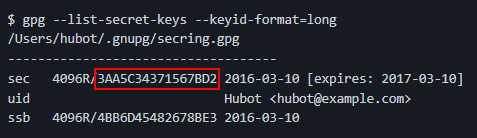
\includegraphics{images/gpg_keys.png}
            \caption{List of \ac{gpg} keys}
            \label{fig:gpg_key}
        \end{figure}
        Copy the \ac{gpg} key ID, in this case: 3AA5C34371567BD2         
        \item Enter this text with your copied ID. Your \ac{gpg} key will be printed to console.
            \begin{lstlisting}[style=bash] 
gpg --armor --export <id>
            \end{lstlisting}
        Copy the printed key, beginning with \textit{BEGIN PGP PUBLIC KEY BLOCK} and ending with \textit{END PGP PUBLIC KEY BLOCK}.  
        \item Now you are able to add the key to your GitHub Account: \url{https://github.com/settings/gpg/new}
        \item \label{itm:gpg_key_end}After you have added the key to GitHub, you have to tell Git your signing key. 
            \begin{lstlisting}[style=bash] 
git config --unset gpg.format
            \end{lstlisting}   
        The \textit{--global} is not necessary in this case. The settings are only made for the current repository you are in. \\
        Use the same \ac{gpg} key id as  in \ref{itm:gpg_key_start} and enter this command. 
            \begin{lstlisting}[style=bash] 
git config user.signingkey <id>
            \end{lstlisting}   
        You can configure Git to sign all commits by default with:
            \begin{lstlisting}[style=bash] 
git config commit.gpgsign true
            \end{lstlisting} 
        From now on, your local commits will be signed.   
        \item Last but not least you have to configure the .bashrc file. It is a startup configuration file for the \ac{bash} which is loaded every time a terminal is opened. The export command will set the environment variable \textit{GPG\_TTY} to the correct terminal so that the passphrase for your \ac{gpg}-key can be queried correctly. The export command will be attached  to the .bashrc file in your home directory.  
            \begin{lstlisting}[style=bash] 
[ -f ~/.bashrc ] && echo 'export GPG_TTY=$(tty)' >> ~/.bashrc
            \end{lstlisting}
    \end{enumerate}
    Once you have successfully completed all the steps, Git is configured in the Docker container.   


\section{How to set up Quarkus for remote development}\label{sec:quarkus_remote}
    This chapter is about setting up Quarkus in a Docker container \autocite[cf.][]{quarkus}. If you have already completed the steps from section \ref{sec:git_remote}, you can continue with this container. Otherwise, you have to create a new container.

    \begin{enumerate}
        \item Install curl because it will be needed in future steps.
        \begin{lstlisting}[style=bash] 
apt-get update; apt-get install -y curl
        \end{lstlisting}
        \item Now you are able to install Quarkus via curl.
        \begin{lstlisting}[style=bash] 
curl -Ls https://sh.jbang.dev | bash -s - trust add https://repo1.maven.org/maven2/io/quarkus/quarkus-cli/
        \end{lstlisting}

        \begin{lstlisting}[style=bash] 
curl -Ls https://sh.jbang.dev | bash -s - app install --fresh --force quarkus@quarkusio
        \end{lstlisting}

        \item When you initially set up Quarkus, you have to create a new Quarkus application. In this case a getting started application would be created in the folder \textit{code-with-quarkus}. You are able to specify parameters to define the build system, for example Maven or Gradle. For more information about the available parameters, execute quarkus create app --help.
        \begin{lstlisting}[style=bash] 
quarkus create && cd code-with-quarkus
        \end{lstlisting}
        \item Set \textit{quarkus.http.host} to 0.0.0.0 in application.properties under src/main/resources.
        \item Now you are able to run your application with:
        \begin{lstlisting}[style=bash]
quarkus dev
        \end{lstlisting}
        When you start the application in dev mode, live coding is active which means that you don't have to restart the application to apply changes.
    \end{enumerate}
    To connect a database to your container (needed in future steps), you have to create a docker network. 
    \begin{lstlisting}[style=bash]
docker network create --driver bridge quarkus-net
    \end{lstlisting}
    Afterwards you are able to attach your container to this network: 
    \begin{lstlisting}[style=bash]
docker network connect quarkus-net <container-name>
    \end{lstlisting}

    \section{How to use the Dockerfile for setup}\label{sec:dockerfile}
        In this section you will get some instructions how to use the Dockerfile to set up the remote development. The Dockerfile is located in the root of the project. 
        Run the following commands in a terminal. 
        \begin{enumerate}
            \item Build a docker image from the provided Dockerfile. You have to replace the tokens <REPLACE-ME> with your credentials and your API-Token:
            \begin{lstlisting}[style=bash]
docker build --build-arg GH_TOKEN=<REPLACE-ME> --build-arg username=<REPLACE-ME> --build-arg email=<REPLACE-ME> -t quarkus_image .
            \end{lstlisting}
            \item \label{item:network} Before you are able to create and run the container, you have to create a seperate network for your container, for example to connect a database (\ref{sec:database}). 
            \begin{lstlisting}[style=bash]
docker network create --driver bridge quarkus-net
            \end{lstlisting}
            \item After you have created your image, you can create a container which is attached to the currently created network:
            \begin{lstlisting}[style=bash]
docker run --network quarkus-net --name quarkus -it quarkus_image
            \end{lstlisting} 
        \end{enumerate}
        The installation of the gpg keys to sign your commits has to be done manually as well but the project provides a generation script \textit{gen-key-script}. Attach to the Quarkus container and follow these steps: 
        \begin{enumerate}
            \item Before executing the generation script you have to replace the \textit{REPLACE-ME}-tokens with your own credentials. Do not forget your passphrase, you will need it for signing your commits. Afterwards you can run the script: 
            \begin{lstlisting}[style=bash]
gpg --batch --gen-key gen-key-script && git checkout gen-key-script
            \end{lstlisting}
            The checkout statement ensures that the file is reset so that the password does not end up in git.
            \item Now you have to tell git and GitHub your signing key. Follow the steps described from \ref{itm:gpg_key_start} to \ref{itm:gpg_key_end} in section \ref{sec:quarkus_remote}.
        \end{enumerate}
        

    \section{Attach Visual Studio Code to Docker Container}\label{sec:attach}
    Open VSCode and navigate to the Docker-symbol in the vertical-left bar as shown in figure \ref{fig:attach_vscode}. \\
    When Docker Desktop is running, you will see all your containers. Maybe you have to start the container first. \\
    Peform a right click on the respective container and select \glqq Attach Visual Studio Code\grqq. 
    \begin{figure}[h]
        \centering
        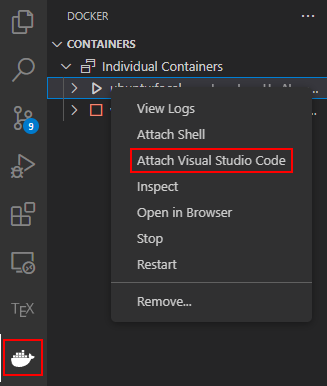
\includegraphics[scale=0.7]{images/attach_VSCode.png}
        \caption{Attach Docker Container to VSCode}
        \label{fig:attach_vscode}
    \end{figure}
    
    Afterwards the container will be attached to VSCode, which can be seen by the green information in the bottom left corner. In figure \ref{fig:container_attached} you can see an example. The text may vary, depending on your image and container name.     
    
    \begin{figure}[h]
        \centering
        
\includegraphics{images/container_attached.png}
        \caption{Docker Container is attched}
        \label{fig:container_attached}
    \end{figure}

    \section{How to set up a database container}\label{sec:database}
        In this section you will get some information how to create a database within a container and connect it to your quarkus container.  
        \begin{enumerate}
            \item Create and run a PostgreSQL database. The quarkus-net network has to be already created (look at step \ref{item:network} in section \ref{sec:dockerfile}):
            \begin{lstlisting}[style=bash]
docker run --rm=true --name hibernate --network quarkus-net -e POSTGRES_USER=hibernate -e POSTGRES_PASSWORD=hibernate -e POSTGRES_DB=hibernate -p 5432:5432 postgres:14.1
            \end{lstlisting}
            \item You will find a file named \textit{.env.example} inside the root of the project. Rename this file to \textit{.env}. This is the place where your environment variables are stored. Make sure that the varibale \textit{POSTGRESQL\_SERVICE\_HOST} is set to \textit{hibernate}. \\
            When you are not developing inside the quarkus container but on your local machine, you have to comment out the mentioned line. 
        \end{enumerate}
        Now your Quarkus container and the database container are in the same network and are able to communicate with each other. 
    
    \section{How to use docker-compose for setup}\label{sec:docker-compose}
        In this section you will get some instructions how to use the \textit{docker-compose.yml} file to set up the remote development. The docker-compose consists of two several parts: the quarkus-dev container and the postgres database container. The manual steps described in \ref{sec:database} for example are not necessary anymore because they will be already included. \\
        The \textit{docker-compose.yml} file is located in the root of the project. Before executing the docker compose command you have to make sure that the corresponding variables in your .env file are set. It is about \textit{GH\_TOKEN}, \textit{uname} and \textit{email}. There is an explanation for the variables in the .env file. When these variables are set you are able to continue.
        \begin{enumerate}
            \item Create and run the containers in background with option -d:
            \begin{lstlisting}[style=bash]
docker compose up -d
            \end{lstlisting}
        \end{enumerate}
        Now the quarkus-dev container and the postgres database container are both running. 
            
        Similar to \ref{sec:dockerfile}, the installation of the gpg keys to sign your commits has to be done manually but the project provides a generation script gen-key-script. Attach to the Quarkus container and follow these steps:
        \begin{enumerate}
            \item Before executing the generation script you have to replace the \textit{REPLACE-ME}-tokens with your own credentials. Do not forget your passphrase, you will need it for signing your commits. Afterwards you can run the script: 
            \begin{lstlisting}[style=bash]
gpg --batch --gen-key gen-key-script && git checkout gen-key-script
            \end{lstlisting}
            The checkout statement ensures that the file is reset so that the password does not end up in git.
            \item Now you have to tell git and GitHub your signing key. Follow the steps described from \ref{itm:gpg_key_start} to \ref{itm:gpg_key_end} in section \ref{sec:quarkus_remote}.
            \end{enumerate}

        You are able to start and stop your container composition with:
        \begin{itemize}
            \item 
                \begin{lstlisting}[style=bash]
docker compose start 
                \end{lstlisting}
                
            \item 
                \begin{lstlisting}[style=bash]
docker compose stop  
                \end{lstlisting}
            \end{itemize}




\chapter{Implementation}
    The microservice will be created with the Java-Framework \textit{Quarkus}. The data is stored in a PostgreSQL database. Hibernate is used as an objectrelational mapper for communicating with the database. \\
    The microservice will be implemented in a hexagonal architecture \autocite[cf.][]{hexagonal_architecture} containing three main folders: application, domain and framework.
    
    \section{Use-Case diagram}
        Figure \ref{fig:use_case} shows the different use cases from the user's point of view. \\
        Creating and updating ball bearings in O-arrangement include the calculation of lifetime. 
        \begin{figure}[h]
            \centering
            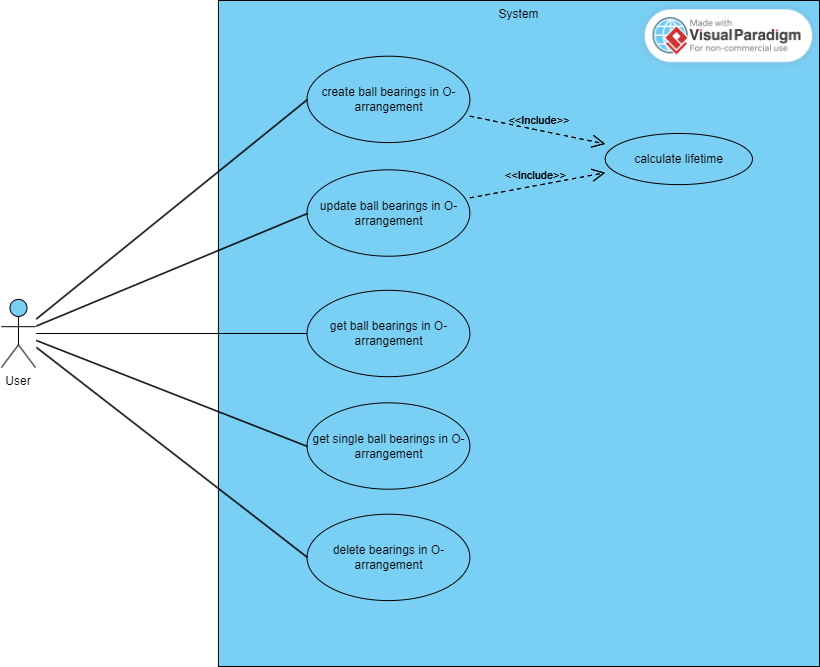
\includegraphics[scale=0.5]{images/use_case_diagram.png}
            \caption{Use-Case diagram}
            \label{fig:use_case}
        \end{figure}
        
        You will notice that the use cases match the implemented test cases (see chapter \ref{sec:testing}).
    
    \section{Structure of the service}
        You can see a list of the provided endpoints in \ref{fig:endpoints}. The service provides the basic CRUD (Create, Read, Update, Delete)-operations while consuming and producing JSON data. 

        \begin{figure}[h]
            \centering
            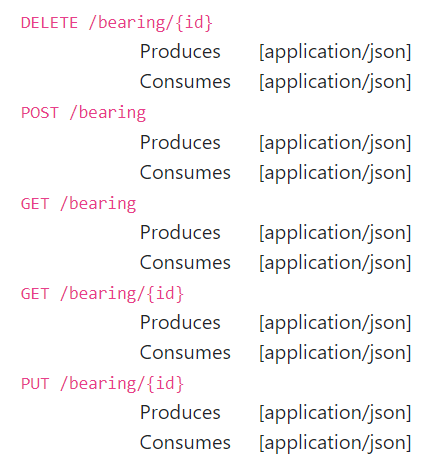
\includegraphics{images/endpoints.png}
            \caption{List of endpoints}
            \label{fig:endpoints}
        \end{figure}

        You can see the plain folder structure including all Java files in image \ref{fig:folder} and \ref{fig:folder_2}. The structure is based on the \textit{hexagonal architecture} presented in book \autocite{hexagonal_architecture}. Chapter \ref{sec:hex-architecture} discusses some important aspects of the \textit{hexagonal architecture}.
        \newpage
        \begin{figure}[h]
            \dirtree{%
            .1 src/main/java/org/dhbw/mosbach/ai/ .
            .2 application/ .
            .3 ports/ .
            .4 input/ .
            .5 OArrangementCommandInputPort.java .
            .5 OArrangementQueryInputPort.java .
            .4 output/ .
            .5 OArrangementDbCommandOutputPort.java .
            .5 OArrangementDbQueryOutputPort.java .
            .3 usecases/ .
            .4 OArrangementCommandUseCase.java .
            .4 OArrangementQueryUseCase.java .
            .2 domain/ .
            .3 entity/ .
            .4 Bearing.java .
            .4 Load.java .
            .4 OArrangement.java .
            .3 vo/ .
            .4 Id.java .
            }
            \caption{Folder structure of source code (part 1)}
            \label{fig:folder}
        \end{figure}
        \newpage       
        
        \begin{figure}[h]
            \dirtree{%
            .1 src/main/java/org/dhbw/mosbach/ai/ .
            .2 framework/ .
            .3 adapters/ .
            .4 input/ .
            .5 rest/ .
            .6 request/ .
            .7 CreateBearing.java .
            .7 CreateLoad.java .
            .7 CreateOArrangement.java .
            .6 OArrangementManagementAdapter.java .
            .4 output/ .
            .5 postgres/ .
            .6 data/ .
            .7 BearingData.java .
            .7 LoadData.java .
            .7 OArrangementData.java .
            .6 mapper/ .
            .7 OArrangementMapper.java .
            .6 repository/ .
            .7 OArrangementRepository.java .
            .6 OArrangementDbCommandPostgresAdapter.java .
            .6 OArrangementDbQueryPostgresAdapter.java .
            }
            \caption{Folder structure of source code (part 2)}
            \label{fig:folder_2}
        \end{figure}
        \newpage

    \section{Hexagonal Architecture} \label{sec:hex-architecture}
        "Create your application to work without either a UI or a database so that you can run automated regression tests against the application, work when the database becomes unavailable, and link applications together without any user involvement" (Alistair Cockburn). \\
        This quote lays the groundwork for understanding hexagonal architecture.

        The individual components of the hexagonal architecture are shown in Figure \ref{fig:hex-architecture}. The architecture was adopted 1 to 1 in the folder structure in figure \ref{fig:folder} and  \ref{fig:folder_2}. 

        \begin{figure}[h]
            \centering
            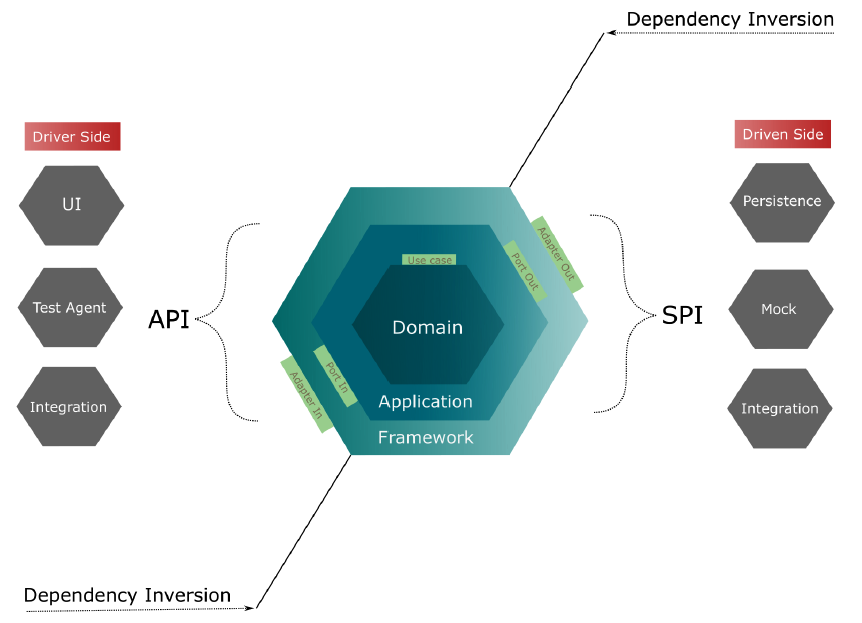
\includegraphics[scale=0.75]{images/hex-architecture.png}
            \caption{Hexagonal Architecture}
            \mbox{(Source: \autocite[][p.13]{hexagonal_architecture})}
            \label{fig:hex-architecture}
        \end{figure}

        One of the main ideas of the hexagonal architecture is to separate business code from technology code \autocite[cf.][p.]{hexagonal_architecture}. You have to be able to change technology code without affecting business logic. The architecture consists of different hexagons (see figure \ref{fig:hex-architecture}). One of them is the \textbf{Domain hexagon}. In the Domain hexagon, we assemble the elements responsible for describing the core problems we want our software to solve. Entities and \ac{vo} are the main elements that are utilized in the Domain hexagon. This part corresponds to the folder domain/ in figure \ref{fig:folder}. Entities represent things we can assign an identity to, and value objects are immutable components that we can use to build our entities. \\
        The \textbf{Application hexagon} sits between the business and technology sides, serving as a middleman to interact with both parties. It utilizes ports and use cases to perform its functions (see figure \ref{fig:application-hexagon}). 

        \begin{figure}[h]
            \centering
            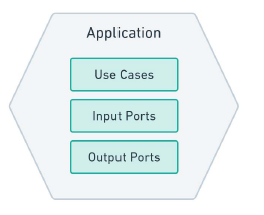
\includegraphics{images/application-hexagon.png}
            \caption{Application hexagon}
            \mbox{(Source: \autocite[][p.17]{hexagonal_architecture})}
            \label{fig:application-hexagon}
        \end{figure}

        Use cases represent the system's behavior through application-specific operations. You can represent use cases as abstractions defined by interfaces. \\
        An input port is the corresponding implementation of a use case interface. \\
        There are situations in which a use case needs to fetch data from external resources (for example a database). That's the role of output ports, which are represented as interfaces. They describe  which kind of data a use case or input port needs to get from outside to perform its operations. 

        The \textbf{Framework hexagon} (see \ref{fig:framework-hexagon}) provides the outside world interface. That's the place where you have the opportunity to determine how to expose application features. This is where you define REST-endpoints, for example. And to consume things from external sources, you use the Framework hexagon to specify the mechanisms to fetch data from databases or any other system. 
        
        \begin{figure}[h]
            \centering
            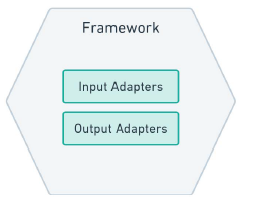
\includegraphics{images/framework-hexagon.png}
            \caption{Framework hexagon}
            \mbox{(Source: \autocite[][p.19]{hexagonal_architecture})}
            \label{fig:framework-hexagon}
        \end{figure}

        In the Framework hexagon you need to decide which technologies should be allowed to communicate with your software. That communication can occur in two forms, one known as driving
        and another known as driven. For the driver side, we use \textbf{Input Adapters}, and for the driven side, we use \textbf{Output Adapters}. \\
        Driving operations are requesting actions to the software, for example a user with a frontend application (in this case: REST-API). As you can see in figure \ref{fig:hex-architecture} the communication occurs through an \ac{api} built on top of the input adapters. \\
        On the other side we have driven operations. These operations are triggered from your application and go into the outside world (for example database). These adapters must conform to our output ports by implementing them.
        
        The use of a hexagonal architecture makes the software much easier to maintain. For example if it's necessary to change some business rule, you only have to change the Domain hexagon.
        \newpage

    \section{Testing the service} \label{sec:testing}
        \textit{REST-assured} and \textit{quarkus-junit5} are used for testing the service. A test was implemented for each endpoint (see \ref{fig:testing}). 

        \begin{figure}[h]
            \centering
            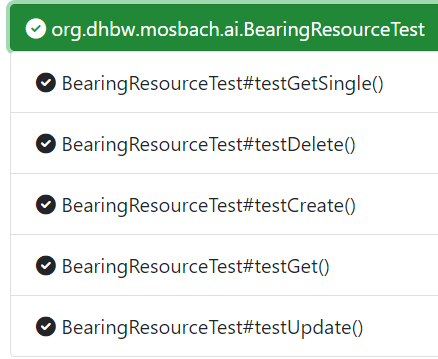
\includegraphics{images/testing.png}
            \caption{List of test cases}
            \label{fig:testing}
        \end{figure}


        As you can see in figure \ref{fig:folder_test} the test cases are located in one test file.
        \begin{figure}[h]
            \dirtree{%
            .1 src/test/java/org/dhbw/mosbach/ai/ .
            .2 BearingResourceTest.java .
            }
            \caption{Folder structure of test code}
            \label{fig:folder_test}
        \end{figure}

        The test cases are consistent with the use cases shown in figure \ref{fig:use_case}.

        


\chapter{Conclusion} % Fazit


	
	\backmatter
	
	% \pagenumbering{roman}
	\frontmatter

	\setcounter{page}{\value{anhangcounter}}
	
	\cleardoublepage
	\phantomsection\addcontentsline{toc}{chapter}{Literature}
	\printbibliography
	
	\chapter{Anhang}
	
\end{document}